\section{Théorie}

\begin{wrapfigure}{R}{0.5\linewidth}
    \centering
    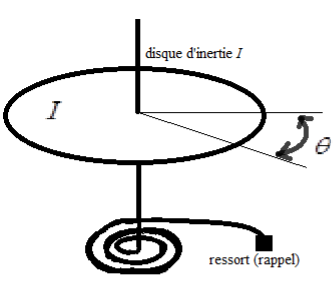
\includegraphics[width=\linewidth]{figures/montage.png}
    \caption{Montage expérimental \cite{notice}}
    \label{fig:montage_exp}
\end{wrapfigure}

Le système étudié est un disque de moment d'inertie \(I\) contraint à tourner selon son axe. La \autoref{fig:montage_exp} montre en plus de détails le montage. \(\theta\) est l'angle de rotation du disque. Un système d'amortissement magnétique permet de changer la force de frottement, proportionelle à \(\dot \theta\), subie par le disque. Cette force applique un moment de force \(\overrightarrow{M_\textrm{frot}} = -N \dot\theta \vec{e_z}\), où \(N\) est le coefficient du couple de frottement. De plus, un ressort applique une force de rappel le long de l'axe du disque, résultant en un moment de forces \(\overrightarrow{M_\textrm{rappel}} = -k \theta \vec{e_z}\), où \(k\) est la constante du couple de rappel. L'excitation periodique du ressort par un moteur applique un couple dépendant du temps \(G(t)\), donnant \(\overrightarrow{M_\textrm{excit}} = G(t) \vec{e_z}\). Par le théorème du moment d'inertie:
\begin{equation}
    \frac{\dd L}{\dd t} = I \ddot \theta = M_\textrm{tot} = G(t) - N \dot\theta - k\theta
    \label{eq:theoreme_moment_inertie}
\end{equation}
En définissant
\begin{itemize}
    \item \(\lambda = \frac{N}{2I}\) le coefficient d'amortissement,
    \item \(\omega_0 = \sqrt{\frac{k}{I}}\) la pulsation de l'oscillateur harmonique
    \item \(\frac{G(t)}{I} = p \sin (\Omega t)\), où \(p\) et \(\Omega\) sont respectivement l'amplitude et la fréquence de la perturbation
\end{itemize}
il est possible de réécrire l'\autoref{eq:theoreme_moment_inertie} comme:
\begin{equation}
    \ddot\theta + 2\lambda\dot\theta + \omega_0^2\theta = p \sin (\Omega t)
    \label{eq:mouvement}
\end{equation}
ce qui donne l'équation différentielle de l'oscillateur harmonique, qu'il est possible de résoudre à partir des conditions initiales.

\paragraph*{Oscillations libres}
L'oscillation est dite "libre" si le couple forcant n'est pas appliqué, c'est à dire \(p = 0\). À partir des conditions initiales \(\theta(0) = \theta_0\) et \(\dot\theta(0) = 0\), il est possible de trouver 3 solutions en fonction des valeurs de \(\omega_0\) et \(\lambda\):
\begin{equation}
    \begin{cases}
        \begin{aligned}
            &\theta(t) = \theta_0 e^{-\lambda t} \cos (\omega t + \phi) &&\textrm{si } \lambda^2 < \omega_0^2, \textrm{où } \omega^2 = \omega_0^2 - \lambda^2 \\
            &\theta(t) = \theta_0 e^{-\lambda t} (1 + \lambda t) &&\textrm{si } \lambda^2 = \omega_0^2 \\
            &\theta(t) = \theta_0 e^{-\lambda t} \left(C_1e^{\omega t} + C_2e^{-\omega t}\right) &&\textrm{si } \lambda^2 < \omega_0^2, \textrm{où } \omega^2 = \lambda^2 - \omega_0^2
        \end{aligned}
    \end{cases}
\end{equation}
Pour cette expérience, seul le cas de l'amortissment faible avec \(\lambda^2 < \omega_0^2\) sera considéré. \(\phi\) est une constante donnant la phase de l'oscillation.

\paragraph*{Oscillations forcées}
Pour cette section, la situation \(p \ne 0\), c'est à dire la présence d'un couple sinusoïdal, sera considérée. Pour le cas de l'amortissement faible, la solution de l'\autoref{eq:mouvement} devient:
\begin{equation}
    \theta(t) = A(\Omega) \sin(\Omega t + \psi) + C e^{-\lambda t} \cos(\omega t - \phi)
    \label{eq:oscillations_forcees}
\end{equation}

\begin{wrapfigure}{R}{0.3\linewidth}
    \vspace*{-0.5cm}
    \centering
    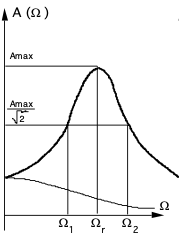
\includegraphics[width=\linewidth]{figures/pic_amplitude.png}
    \caption{Amplitude des oscillations en fonction de la pulsation \cite{notice}}
    \label{fig:pic_amplitude}
\end{wrapfigure}
où \(\omega = \omega_0^2 - \lambda^2\), 
\begin{equation}
    A(\Omega) = \frac{p}{\sqrt{\left(\omega_0^2-\Omega^2\right)^2 + 4\lambda^2\Omega^2}}, \quad \psi = \arctan \left(\frac{2\lambda\Omega}{\omega_0^2-\Omega^2}\right)
\end{equation}

L'amplitude \(A(\Omega)\) est maximale autour de la pulsation de résonnance \(\Omega_r = \sqrt{\omega_0^2-2\lambda^2}\). Cette situation est illustrée sur la \autoref{fig:pic_amplitude}. La largeur du pic d'amplitude à mi-hauteur peut être définie comme \(\Delta \Omega = \frac{2 \lambda \omega}{\Omega_r}\). De plus, ces valeurs permettent de définir le facteur de qualité de résonnance, qui vaut \(Q = \frac{\Omega_r}{\Delta\Omega}\).

\paragraph*{Régime transitoire}
De l'\autoref{eq:oscillations_forcees}, il est possible de voir que pour un \(t\) croissant, le second terme perd de l'importance dans le temps. Cela correspond au régime transitoire. Si \(\Omega\) et \(\omega\) sont proches, un battement de pulsation \(\omega_B = |\omega- \Omega|\) se produit.
